
\begin{obs}\textbf{Extensión del Teorema de Green.} \label{obs:extension_green}
El teorema de Green es aplicable a regiones aún más generales que las simplemente conexas. Dicho teorema puede ser adaptado a cualquier región en $\Rn{2}$ cuya frontera se pueda descomponer en un número finito de curvas cerradas y simples. La idea es ``recorrer'' dicha frontera pasando por todas las curvas que la conforman, garantizando que la región siempre quede a la izquierda del sentido de recorrido.
\end{obs}

Veamos, a modo ilustrativo,  el siguiente ejemplo. Sea $D \subset \mathbb{R}^{2}$   el siguiente conjunto (pintado de violeta),  claramente $D$  no simplemente conexo. 
    
   

\begin{center}
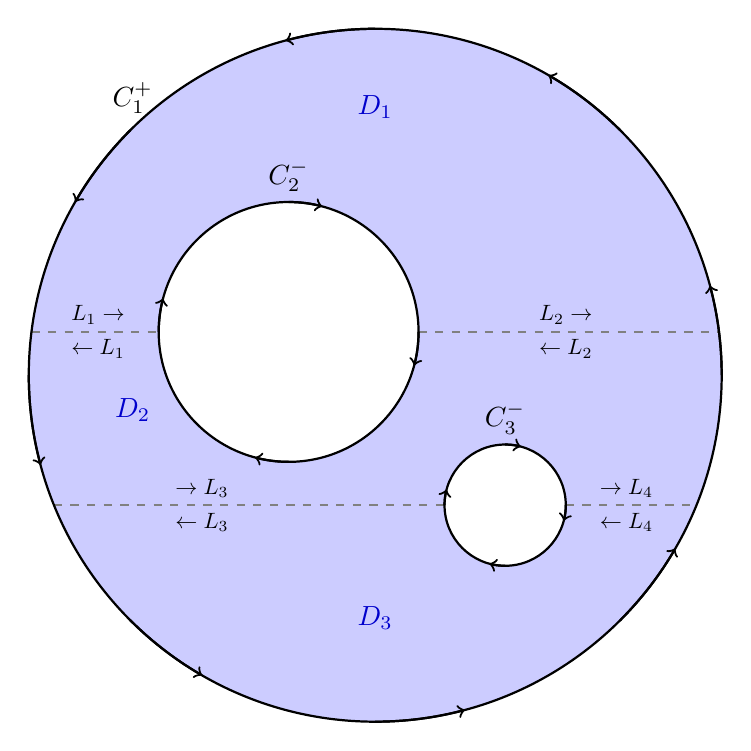
\begin{tikzpicture}[scale=1.1]
    % 1. REGION AZUL (Fondo de toda la figura)
    \fill[blue!20] (0,0) circle (4);
    
    % 2. VACIADO DE LOS AGUJEROS INTERIORES (En blanco)
    \fill[white] (-1,0.5) circle (1.5);
    \fill[white] (1.5,-1.5) circle (0.7);

    % 3. LÍNEAS DE CORTE TRANSVERSALES (Dashed)
    % Línea superior corregida: pasa por el centro de C_1 (y = 0.5)
    % Tramo izquierdo (desde el borde exterior hasta el inicio de C_1)
    \draw[thick, dashed, gray] (-3.97, 0.5) -- (-2.5, 0.5); 
    % Tramo derecho (desde el final de C_1 hasta el borde exterior)
    \draw[thick, dashed, gray] (0.5, 0.5) -- (3.97, 0.5); 
    
    % Línea inferior: pasa por el centro de C_2 (y = -1.5)
    % Tramo izquierdo (desde el borde exterior hasta el inicio de C_2)
    \draw[thick, dashed, gray] (-3.71, -1.5) -- (0.8, -1.5);
    % Tramo derecho (desde el final de C_2 hasta el borde exterior)
    \draw[thick, dashed, gray] (2.2, -1.5) -- (3.71, -1.5);

    % 4. BORDE EXTERIOR C - ¡ORIENTACIÓN ANTIHORARIA!
    \draw[thick] (0,0) circle (4);
    \foreach \angle in {0, 45, 90, 135, 180, 225, 270, 315} {
        \draw[thick, ->] ({4*cos(\angle)}, {4*sin(\angle)}) arc[start angle=\angle, end angle=\angle+15, radius=4];
    }
    
    % 5. AGUJERO INTERIOR C_1 - ¡ORIENTACIÓN HORARIA!
    \draw[thick] (-1,0.5) circle (1.5);
    \foreach \angle in {0, 90, 180, 270} {
        \draw[thick, ->] ({-1+1.5*cos(\angle)}, {0.5+1.5*sin(\angle)}) arc[start angle=\angle, end angle=\angle-15, radius=1.5];
    }
    
    % 6. AGUJERO INTERIOR C_2 - ¡ORIENTACIÓN HORARIA!
    \draw[thick] (1.5,-1.5) circle (0.7);
    \foreach \angle in {0, 90, 180, 270} {
        \draw[thick, ->] ({1.5+0.7*cos(\angle)}, {-1.5+0.7*sin(\angle)}) arc[start angle=\angle, end angle=\angle-15, radius=0.7];
    }

    % 7. ETIQUETAS DE SUBREGIONES SIMPLEMENTE CONEXAS
    \node[blue!80!black] at (0,3.1) {$D_1$};  
    \node[blue!80!black] at (-2.8, -0.4) {$D_2$};  % Se movió el nodo D_2 a la derecha para que no se pise con la línea
    \node[blue!80!black] at (0,-2.8) {$D_3$};  

    % 8. ETIQUETAS DE CURVAS DE FRONTERA
    \node at (-2.8, 3.2) {$C_1^{+}$};
    \node at (-1, 2.3) {$C^{-}_2$};  % Se subió la etiqueta C_1 para que quede dentro del blanco y libre de la línea
    \node at (1.5, -0.5) {$C^{-}_3$}; 

    % 9. ETIQUETAS DE LOS CORTES L_i (Calibradas a las alturas reales de los centros)
    % Corte Superior Izquierda (L_1)
    \node[above, scale=0.8] at (-3.2, 0.5){$L_1 \rightarrow$} ;
    \node[below, scale=0.8] at (-3.2, 0.5) {$\leftarrow L_1$};
    
    % Corte Superior Derecha (L_2)
    \node[above, scale=0.8] at (2.2, 0.5) {$L_2 \rightarrow$};
    \node[below, scale=0.8] at (2.2, 0.5) {$\leftarrow L_2$};
    
    % Corte Inferior Izquierda (L_3)
    \node[above, scale=0.8] at (-2.0, -1.5) {$\rightarrow L_3$};
    \node[below, scale=0.8] at (-2.0, -1.5) {$\leftarrow L_3$};
    
    % Corte Inferior Derecha (L_4)
    \node[above, scale=0.8] at (2.9, -1.5) {$\rightarrow L_4$};
    \node[below, scale=0.8] at (2.9, -1.5) {$\leftarrow L_4$};

\end{tikzpicture}
\end{center}
 

El conjunto $D$ puede ser escrito como la uni\'on de tres conjuntos  simplemente conexos y  disjuntos entre si (salvo tal vez en sus bordes),   $D_1$, $D_2$ y $D_3$, es decir,  $$D =D_1\cup D_2\cup D_3.$$  El borde de $D$ es la uni\'on de tres curvas cerradas simples,   $C1$, $C_2$ y $C_3$, es decir,  $$\partial D=C_1\cup C_2\cup C_3.$$


Se deja como tarea al lector probar que:  
\[ 
  \iint_D \grad\times\mathbf{F}\cdot dA = \oint_{C_1^{+}}\mathbf{F}\cdot d\mathbf{s} + \oint_{C_2^{-}}\mathbf{F}\cdot d\mathbf{s} + \oint_{C_3^{-}}\mathbf{F}\cdot d\mathbf{s}
\]



\begin{theorem} \textbf{Generalización a Regiones con Múltiples Fronteras} Si la región \(D\) tiene una frontera exterior \(C_{1}\) y fronteras interiores \(C_2, C_3, \dots, C_n\) (todas orientadas positivamente respecto a \(D\) y disjuntas dos a dos), el teorema se expresa como:\[ \iint_D \grad\times\mathbf{F}  \: dA=  \oint _{C_{1}}  \mathbf{F}\cdot d\mathbf{s} -  \sum _{i=2}^{n} \oint _{C_{i}}    \mathbf{F}\cdot d\mathbf{s}  \]
\end{theorem}





\begin{tarea}
Sea $F(x,y) = (\dfrac{y}{x^{2}+y^{2}},\dfrac{-x}{x^{2}+y^{2}})$ y sea $C$ una curva en el plano, cerrada, simple y orientada en sentido antihorario. Calcular todos  los posibles valores de $\int_{C} F ds.$
\end{tarea}